\chapter{Functional Implementation Through Kanban Increments}

\section*{Introduction}
This chapter presents implementation as a sequence of value-oriented Kanban increments. The increments are reporting groupings, not time-boxed sprints. Each one combines requirements, backend behavior, frontend interaction, and validation considerations.

\section{Increment 1: Foundation, Identity, and Centers}
\subsection{Objective and Scope}
The first increment established the application skeleton, user identity, protected routing, and donation-center foundation. These capabilities were prerequisites for all role-aware workflows.

On the backend, authentication and user concerns integrate Spring Security, token handling, validation, and persistence. Center modules provide command and query use cases, mappers, repository adapters, slot management, staff profiles, operating hours, closures, and administrative controllers. On the frontend, authentication pages cover registration, login, verification, forgotten password, and reset. Center routes and services expose listing, detail, creation, and management views.

\subsection{Design Decisions}
Email verification separates account creation from trusted access. Password reset uses short-lived proof rather than exposing or transmitting an existing password. Center registration and approval are separate because submission by a center actor does not imply platform authorization. Staff membership is modeled explicitly so that access can be limited to a center.

\uiscreenshotpair{assets/5.1/auth/auth-login.png}{Donor sign-in}{assets/5.1/auth/verification-success.png}{Successful email verification}{Login and account verification interfaces}{ui-authentication}
\uiscreenshotpair{assets/5.1/center/centers-map.png}{Geographic center discovery}{assets/5.1/center/centers-list.png}{Searchable center list}{Donation-center discovery interfaces}{ui-center-discovery}
\uiscreenshotpair{assets/5.1/center/create-center.png}{Center registration form}{assets/5.1/center/center-approval.png}{Administrative approval queue}{Center registration and approval interfaces}{ui-center-approval}

\subsection{Acceptance Scenarios}
\begin{itemize}
  \item a new user can register and verify the account before protected use;
  \item invalid credentials or expired reset proof are rejected without revealing sensitive detail;
  \item public users can consult approved center information;
  \item a center registration remains pending until authorized approval;
  \item a center administrator can manage only the relevant center and staff.
\end{itemize}

\section{Increment 2: Donor Profiles and Appointments}
\subsection{Objective and Scope}
The second increment enabled donors to complete the information required for safe coordination and reserve center capacity. The donor module includes profile, health questionnaire, blood type, location, availability, history, eligibility, certificate, and impact responsibilities. The appointment module includes creation, rescheduling, cancellation, status, health screening, and outcome.

The Angular application provides onboarding pages for health, blood type, location, availability, and notification preferences. It also provides center detail, slot booking, appointment cards, and donor dashboard views. MapLibre supports map display without making location an untyped UI string.

\subsection{Workflow}
The donor selects a center and date, receives available slots, and submits a booking. The backend verifies identity, donor state, center/slot validity, and conflicts. A successful response becomes part of the donor history and center schedule. Rescheduling repeats validation against the target slot.

\uiscreenshotpair{assets/5.2/donor/onboarding.png}{Health-screening questionnaire}{assets/5.2/donor/blood-location.png}{Blood type and location step}{Donor onboarding workflow}{ui-donor-onboarding}
\uiscreenshot{assets/5.2/donor/preferences.png}{Notification-preference configuration}{ui-donor-preferences}
\uiscreenshotpair{assets/5.2/appointment/center-selection.png}{Donation-center selection}{assets/5.2/appointment/time-slot-selection.png}{Date and available-slot selection}{Appointment center and slot selection}{ui-appointment-selection}
\uiscreenshot{assets/5.2/appointment/confirmation.png}{Appointment booking confirmation}{ui-appointment-confirmation}

\subsection{Privacy Considerations}
Health answers and precise location must not be included in generic list responses. The UI should explain why data is collected and allow notification preferences to be changed. Location improves proximity matching but should not be treated as public profile information.

\section{Increment 3: Staff Operations and Donation Completion}
\subsection{Objective and Scope}
This increment connected planned appointments to actual center operations. Staff need a daily schedule and a focused task queue. At arrival, the staff member checks in the donor, consults authorized eligibility information, records screening, and completes or rejects the donation outcome.

The screening record captures the decision at donation time. It does not replace professional medical judgment. Completing an appointment can update donation history and future eligibility. Marking a donor as no-show can contribute to reliability logic, but automatic penalties should remain transparent and correctable.

\subsection{Operational Sequence}
The staff interface should prioritize today's records, status, scheduled time, and next action. QR-code support can accelerate check-in, but the decoded identifier must still be authorized and validated by the backend. A QR code is a pointer, not proof of eligibility.

\uiscreenshotpair{assets/5.3/staff-queue/scheduled-queue.png}{Scheduled donor queue}{assets/5.3/staff-queue/appointment-check-in.png}{Appointment check-in list}{Center staff schedule and check-in interfaces}{ui-staff-checkin}
\uiscreenshotpair{assets/5.3/staff-queue/qr-check-in.png}{QR-assisted check-in}{assets/5.3/staff-queue/checked-in-queue.png}{Checked-in donor ready for screening}{QR check-in and staff processing queue}{ui-qr-checkin}
\uiscreenshot{assets/5.3/staff-queue/screening.png}{Health screening form}{ui-health-screening}

\subsection{Auditability}
Screening, completion, no-show, and staff administration are state-changing actions. Audit records should capture the authenticated actor, action, target, timestamp, and safe metadata. Sensitive questionnaire content should not be copied wholesale into generic audit text.

\section{Increment 4: Emergency Management}
\subsection{Objective and Scope}
An emergency record expresses a need that cannot wait for normal appointment discovery. It includes required blood information, location, deadline, and lifecycle status. Authorized users create the request, follow its progress, and resolve or expire it. Donors receive only relevant information required to make an informed response.

\diagram[0.44\textheight]{emergency-sequence}{Emergency creation, candidate matching, and response sequence}

The emergency lifecycle must prevent invalid transitions. A resolved or expired request should not continue dispatching new alerts. Acceptance by a donor is not equivalent to a completed donation; it indicates intent and supports coordination. Clinical compatibility and screening remain center responsibilities.

\uiscreenshotpair{assets/5.4/emergencies/emergency-list.png}{Emergency request list}{assets/5.4/emergencies/create-emergency.png}{Emergency creation form}{Emergency management and request creation}{ui-emergency-creation}
\uiscreenshotpair{assets/5.4/emergencies/emergency-details.png}{Emergency progress and response summary}{assets/5.4/donor-response/response-creation.png}{Donor response and slot selection}{Emergency progress and donor-response workflow}{ui-emergency-response}

\section{Increment 5: Matching and Notifications}
\subsection{Objective and Scope}
The fifth increment transformed an emergency into targeted communication. Matching considers blood compatibility, availability, eligibility, geographical distance, and reliability-related information. Candidates are ranked and processed in tiers. If the response is insufficient, the search radius can expand until a configured limit or deadline is reached.

Notification work is transferred through Kafka so that API response time is not coupled to delivery channels. The notification service can persist delivery state, apply preferences, and deliver real-time updates over WebSocket. Failure is observable and retryable without recreating the emergency.

\clearpage
\begin{figure}[H]
\centering
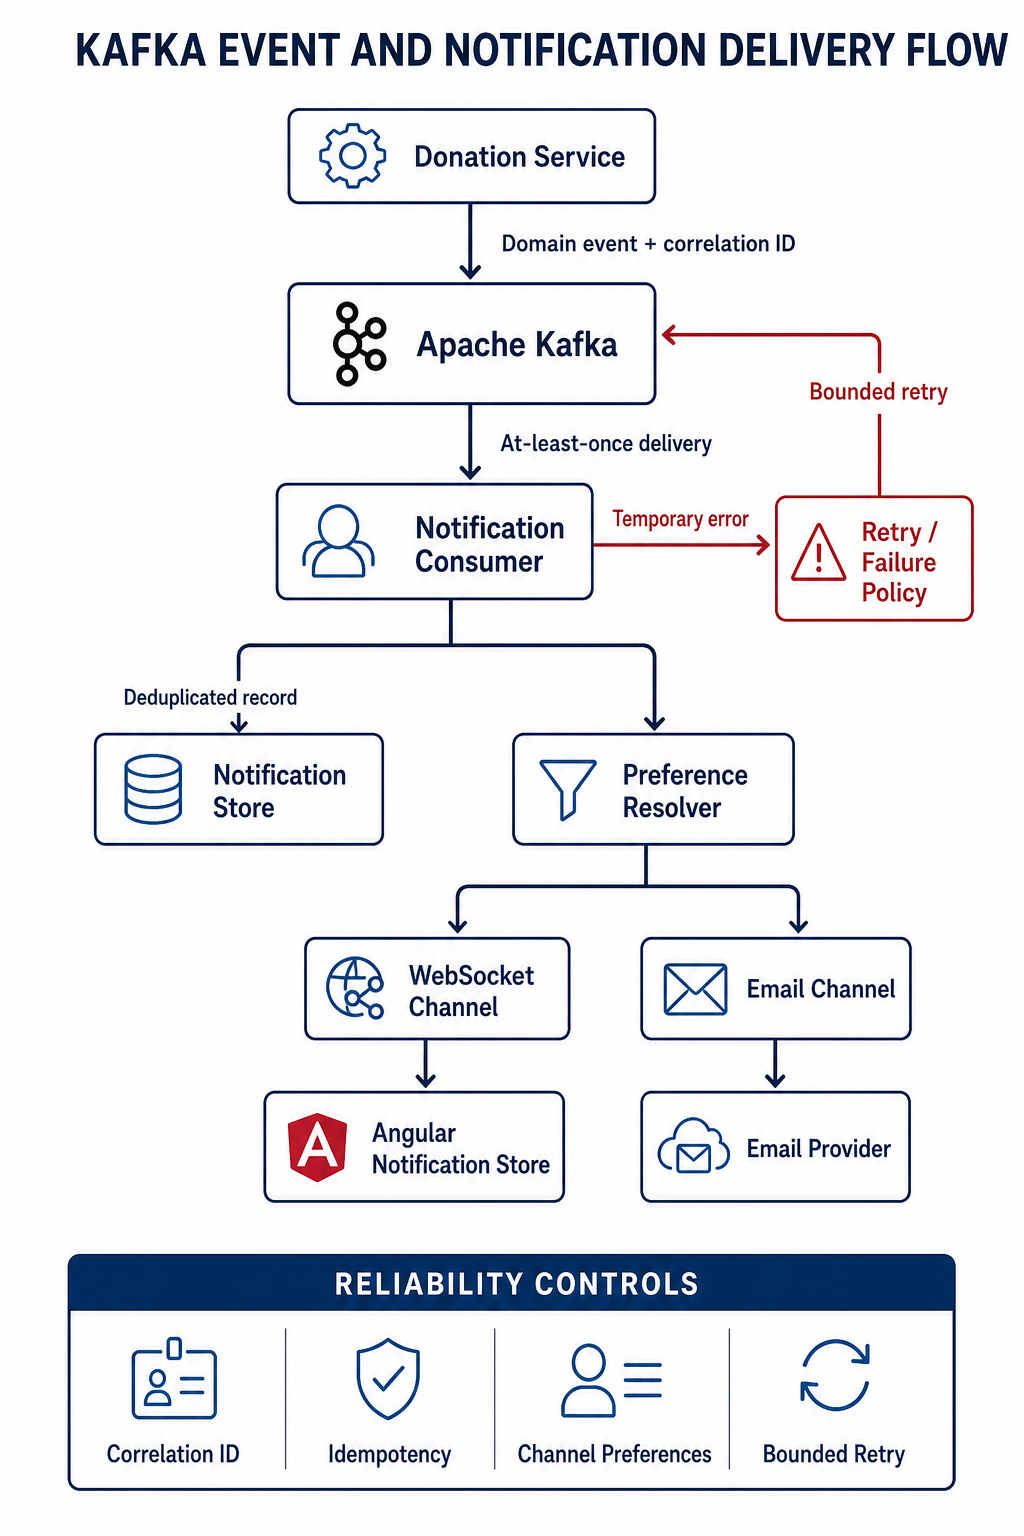
\includegraphics[width=0.82\textwidth,height=0.73\textheight,keepaspectratio]{assets/generated/kafka-notification-flow-portrait.png}
\caption{Kafka event and notification delivery flow}
\label{fig:notification-event-flow}
\end{figure}

\uiscreenshotpair{assets/5.5/notifications/notifications-center.png}{Emergency alerts in the notification center}{assets/5.4/donor-response/rejection.png}{Controlled emergency-decline dialog}{Donor emergency alert and response interfaces}{ui-emergency-alert}
\uiscreenshotpair{assets/5.5/notifications/notification-popup.png}{Header notification popup}{assets/5.5/notifications/emergency-details.png}{Donor emergency details}{Notification access and emergency-status interfaces}{ui-notification-center}

\section{Increment 6: Analytics, Administration, and Operations}
The final grouping completed cross-cutting administrative and operational capabilities. Center administrators consult activity and analytics, manage staff and slots, and generate reports. Super administrators govern users, roles, center approvals, health restrictions, deletion requests, system dashboards, and audit logs.

Analytics must distinguish operational summaries from clinical prediction. Counts of appointments, completed donations, no-shows, active emergencies, and delivery states can be calculated from platform records. Claims about regional blood demand or medical impact require validated data and are treated as future analytical work when evidence is absent.

\uiscreenshotpair{assets/5.5/super-admin/this-month-analytics.png}{Current-month operational indicators}{assets/5.5/super-admin/all-time-analytics.png}{All-time operational indicators}{Super-administration analytics dashboards}{ui-admin-analytics}
\uiscreenshot{assets/5.5/super-admin/logs.png}{Super-administration audit log interface}{ui-admin-audit}

The same increment includes deployable containers, k3s manifests, CI workflows, and observability configuration. These do not appear directly in a donor workflow, but they determine whether the service can be maintained and diagnosed.

\section{Increment Review}
\begin{table}[H]
\centering\small
\begin{tabularx}{\textwidth}{|P{2.0cm}|P{4.0cm}|Y|Y|}
\hline
\rowcolor{tableheader}\textbf{Increment} & \textbf{User value} & \textbf{Principal dependency} & \textbf{Residual risk}\\ \hline
1 & Trusted users and managed centers & Security and center domain & Verification and authorization edge cases\\ \hline
2 & Donor readiness and planned visits & Identity, centers, slots & Concurrent booking and health privacy\\ \hline
3 & Executed donation workflow & Appointments and staff roles & Screening correctness and audit scope\\ \hline
4 & Trackable urgent request & Donor and center data & Invalid transitions and deadline handling\\ \hline
5 & Targeted, decoupled alerts & Emergency events and preferences & Duplicate delivery and retry exhaustion\\ \hline
6 & Governance and operability & All domain records and deployment & Evidence depth and production hardening\\ \hline
\end{tabularx}
\caption{Kanban increment review and residual risks}
\label{tab:increment-review}
\end{table}

\section*{Conclusion}
The increments trace a dependency-aware path from identity to emergency coordination and operations. Chapter 6 examines donor matching and reliable notification in depth.
